

%%%%%%%%%%%%%%%%%%%%%%%%%%%%%%%%%%%%%%%%%%%%%%%%%%%%%%%%%%%%%%%%%%%%%
\royslide{Outline}{
\tableofcontents
%  \begin{picture}(1,1)
%    \put(200,-15){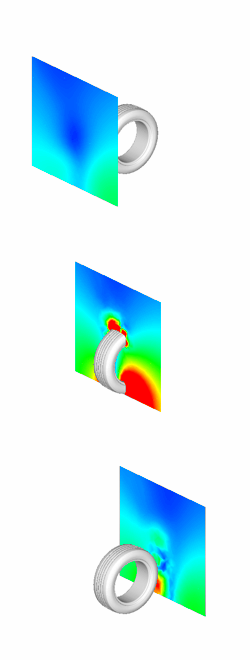
\includegraphics[viewport=0 0 150 660,clip=true,width=.4\textwidth]{figs/tire_rolling_combined}}
%  \end{picture}
}


%\section{Goals}
%
%%%%%%%%%%%%%%%%%%%%%%%%%%%%%%%%%%%%%%%%%%%%%%%%%%%%%%%%%%%%%%%%%%%%%
%\royslide{Goals}{
%
%\begin{itemize}
%\item General frameworks for transient boundary value problems
%\item Adaptive refinement/coarsening strategies
%\item Adaptive mesh refinement/coarsening with general elements
%\item Application studies with adaptive $C^1$ elements
%\end{itemize}
%
%}
